

We now investigate whether word orders as found in natural language reflect optimizization for the memory-surprisal tradeoff.
To this end, we compare the memory-surprisal tradeoffs of 52 actual languages to those of counterfactual reorderings.
We compare to counterfactual reorderings that differ from the actual languages in their word order rules, i.e., the rules that determine how syntactic structures are ordered into strings of words.
To create such counterfactual reorderings, we parameterize these word order rules using a method introduced by Gildea and colleagues \citep{gildea-optimizing-2007, gildea-grammars-2010, gildea-human-2015}:
We construct counterfactual ordering grammars that define consistent ordering rules similar to those found in actual languages.
For instance, these grammars will specify which dependents precede or follow their heads (e.g., whether objects follow or precede verbs, whether adjectives follow or precede nouns), and the relative order of different dependents on the same side of the head (e.g., whether noun phrases have order adjective-numeral-noun or numeral-adjective-noun).

\begin{figure}
\centering
\begin{dependency}[theme = simple]
   \begin{deptext}[column sep=1em]
	   I \&	   wrote \& risāla \& li \& sadīq  \\
   \end{deptext}
	%   \deproot{3}{ROOT}
   \depedge{1}{2}{obj}
	%   \depedge[edge start x offset=-6pt]{2}{5}{ATT}
   \depedge{1}{4}{obl}
   \depedge{4}{3}{case}
   %\depedge[arc angle=50]{7}{6}{ATT}
\end{dependency}
	\caption{TODO Dependencies example}\label{fig:dependency}
\end{figure}


\subsection{Data}
We draw on corpora annotated with syntactic structures.
The Universal Dependencies project has compiled such annotated corpora for several dozen languages~\citep{nivre-universal-2017}.
These are annotated in the format of Dependency Grammar.

\paragraph{Dependency Grammar}
In dependency corpora, sentences are annotated with \emph{dependency trees} (Figure~\ref{fig:dependency}).
These are directed trees describing the grammatical relations among words. For example, the arcs labeled ``obj'' represent that the noun in question is the \emph{direct object} if the verb, rather than e.g. the subject or an indirect object.
A dependency arc is drawn from a \emph{head} (e.g. TODO in Figure TODO) to a \emph{dependent} (e.g. TODO).
Dependency trees can be defined in terms of many different syntactic theories \citep{corbett1993heads}.
Although there are some differences in how different formalisms would draw trees for certain sentences, there is broad enough agreement about dependency trees that it has been possible to develop large-scale dependency-annotated corpora of text from dozens of languages \cite{nivre2017universal}.
\mhahn{currently this is taken from the Greenberg paper}

\paragraph{Selection of Languages}
We considered all languages for which there are Universal Dependencies 2.3 treebanks with a total of at least 500 sentences of training data.
We excluded data from historical languages.\footnote{Ancient Greek, Classical Chinese, Coptic, Gothic, Latin, Old Church Slavonic, Old French.}
TODO While running this experiment, data from additional languages became available that also had enough data, through the Universal Dependencies 2.4 release. TODO.
This resulted in 54 languages.

\paragraph{Processing of Corpora}
For each of these languages, we pooled all available corpora in one dataset.
We excluded corpora that primarily contain code-switched text\footnote{Hindi English corpus}, or text created by non-native speakers.\footnote{ESL for English, CFL for Chinese}
Universal Dependencies corpora have a predefined split into \emph{training}, \emph{held-out} (also known as \emph{development}), and \emph{test} partitions.
While larger corpora have all three partitions, smaller corpora often have only some of these partitions.
For most language, we used the predefined data split, separately pooling data from the different partitions. %We did not use the test partitions.
For some languages with little data, there is no predefined training partition, or the training partition is smaller than the other partitions.
In these cases, we redefined the split to obtain more training data:
For these languages, we pooled all the available partitions, used 100 randomly selected sentences as held-out data, and used the remainder as training data.\footnote{This affects Amharic, Armenian, Breton, Buryat, Cantonese, Faroese, Kazakh, Kurmanji, Naija, Thai, and Uyghur.}
For each language, we used the training and held-out sets for estimating the memory-surprisal tradeoff (see Section~\ref{sec:method}).
We provide the sizes of the resulting datasets in Table~\ref{tab:corpora}.



\subsection{Baselines: Counterfactual Ordering Grammars}
We define ordering grammars, small models of the rules by which languages order syntactic structures into sentences.
Our formalism of ordering grammars adapts the method of \cite{gildea-optimizing-2007, gildea-grammars-2010, gildea-human-2015} to the setting of dependency corpora, following \cite{hahn-universals-2020}.




\begin{figure}
\centering
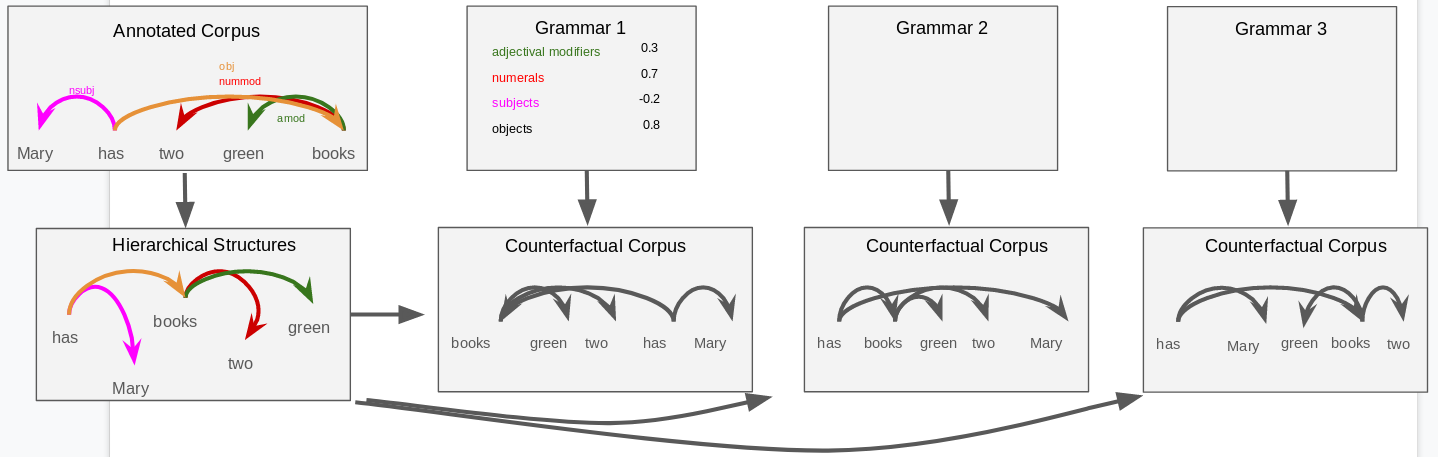
\includegraphics[width=\textwidth]{figures-gdrive/counterfactual-languages.png}
	\caption{\note{Can say more here to explain how it works} Estimating chance by constructing counterfactual grammars and languages.\jd{this figure is again blurry for me. also looks like there's sth in the background on the left?}}\label{fig:grammars}
\end{figure}



Universal Dependencies defines 37 universal syntactic relations that are used to label dependency arcs across all corpora.
These relations encode cross-linguistically meaningful relations such as subjects, objects, and adjectival modifiers.
We define ordering grammars by assigning a parameter $a_\tau \in [-1,1]$ to every one of these 37 universal syntactic relations.
Relations sometimes have language-specific subtypes; we do not distinguish these subtypes.

Following Gildea and colleagues, this parameter defines how dependents are ordered relative to their head:
Given a head and a set of dependents, we order each dependents by the parameter $a_\tau$ assigned to the syntactic relation linking it to the head.
Dependents with negative weights are placed to the left of the head; dependents with positive weights are placed to the right.

Ordering grammars describe languages that have consistent word order:
For instance, the subject is consistently ordered before or after the verb, depending on whether the parameter for the verb-subject dependency is positive or negative.

We construct baseline grammars by randomly sampling the parameters $a_\tau$.
Such baseline grammars define languages that have consistent word order, but do not exhibit preferences for specific word order patterns.


In actual languages, the ordering of words is largely determined by the syntactic relations (CITE).
However, certain kinds of rules cannot be modeled by our word order grammars, such as rules sensitive to the category of the dependent (e.g., differences between nominal and pronominal objects).
Word order freedom also is not modeled.
In this sense, ordering grammars represent approximations to the kinds of ordering rules found in natural language \citep{gildea-optimizing-2007, gildea-grammars-2010, gildea-human-2015}.
See Section (Discussion) for further discussion.



\subsection{Estimating Memory-Surprisal Tradeoff}\label{sec:method}
The key to evaluating the memory-surprisal tradeoff from corpus data is the set of quantities $I_t$.
In order to estimate this, we use LSTM recurrent neural networks (CITE).
Neural network models are the basis of the state-of-the art in statistical modeling of language and in predicting the surprisal effect on reading times~\citep{frank-insensitivity-2011, goodkind-predictive-2018}.
We provide data from more traditional estimation methods in the SI.



\paragraph{Model and Parameter Estimation}
We use a recurrent neural network with Long-Short-Term Memory cells~\citep{hochreiter-long-1997} (CITE for Neural LM).
This architecture takes as input a sequence $x_1 ... x_N$ of words, and at each time $t=1, ..., N$, calculates a probability distribution $p(w_t|w_1...w_{t-1})$ over the next word $w_{t}$ given preceding words $w_1 ... w_{t-1}$.
Our model specification follows (CITE someone who used exactly the same model).

The network is parameterized by a vector $\theta$ of weights determining how the activations of neurons propagate through the network~\citep{hochreiter-long-1997}.
Given a corpus, the numeral parameters of the LSTM are chosen so as to minimize the average surprisal across the training corpus.
%We can think of the LSTM parameters as forming one large vector $\theta$.
At the beginning of training, the parameters $\theta$ are randomly initialized to some setting $\theta_0$.

The training corpus is chopped into word sequences $w_1 ... w_{T_{max}}$ of length ${T_{max}}$, where ${T_{max}}$ is the highest $T$ for which we estimate $I_T$. %  (${T_{max}} = 20$ in our experiments).
We use Stochastic Gradient Descent to optimize the parameters $\theta$ so as to minimize the surprisal
\begin{equation}\label{eq:train}
	\frac{1}{T_{max}} \sum_{i=1}^{T_{max}} \log p_\theta(w_i|w_1...w_{i-1})
\end{equation}
When calculating the parameter update, we use three standard methods of regularization that have been shown to improve neural language modeling: dropout~\citep{srivastava-dropout:-2014}, word dropout, and word noising~\citep{xie2017data}.

Once all sequences have been processed, we start another pass through the training data.
Before each pass through the training data, the order of sentences of the training data is shuffled, and the corpus is again chopped into sequences of length $T$.
After each pass through the training data, the average surprisal~(\ref{eq:train}) at the current parameter setting $\theta$ is evaluated on the held-out partition.
We terminate training once this held-out  surprisal does not improve over the one computed after the previous pass any more.

In our experiments, we chose $T_{max} = 20$. Prior work has found that the probabilities $p(w_t|w_1...w_{t-1})$ are dominated by a small number of preceding words \citep{daniluk2017frustratingly}, suggesting that $I_t$ will be close to zero for $t$ greater than 20.



\paragraph{Choice of Hyperparameters}

The LSTM model has a set of numerical \emph{hyperparameters} that need to be specified before parameter estimation, such as the number of neurons and the learning rate.
See SI for details.
For each corpus, we used Bayesian optimization using the Expected Improvement acquisition function \citep{snoek-practical-2012} to find a good setting of the hyperparameters.
We optimized the hyperparameters to minimize average surprisal~(\ref{eq:train}) on the held-out partition resulting at the end of parameter estimation, on languages generated from random word order grammars.
This biases the hyperparameters towards modeling counterfactual grammars better, biasing them \emph{against} our hypothesis that real orders result in better memory-surprisal tradeoffs than counterfactual orders.

Due to reasons of computational efficiency, neural language models can only process a bounded number of distinct words in a single language (CITE).
For each corpus, we limited the number of distinct processed words to the $N=10,000$ most common words in the training corpus, a common choice for neural language models (CITE).
Following (CITE), we represented other words by their part-of-speech tags as annotated in the corpora.
This applied to 37 languages, affecting an average of 11~\% of words in these languages.
We believe that this modeling limitation does not affect our results for the following reasons.
First, this affects the same words in real and counterfactually ordered sentences.
Second, all excluded words are extremely infrequent in the available data, occurring less than 10 times (except for Czech and Russian, the languages for which we have by far the largest datasets).
Many of the excluded words occur only once in the dataset (78 \% on average across the affected languages).
This means that any model would only be able to extract very limited information about these words from the available training data, likely \emph{less} than what is provided by the part-of-speech tag.
Third, traditional N-gram models, which do not have this limitation, provide results in qualitative agreement with the neural network-based estimates (see SI).




\paragraph{Estimating the Memory-Surprisal Tradeoff Curve}
The quantity $I_t$ in~(\ref{eq:memory-bound}) is equal to the difference 
\begin{equation}
\operatorname{I}[w_t, w_0 | w_1, ..., w_{t-1}] = H[w_t|w_1, ..., w_{t-1}] - H[w_t|w_0, w_1, ..., w_{t-1}]
\end{equation}
This quantity can be estimated as follows.
After estimating the parameter vector $\theta$, we compute the following difference for each word $w_t$ ($t$ ranging from $T_{max}$ up to the length of the held-out partition) in the held-out partition:
\begin{equation}
	\frac{1}{|HeldOut|-t} \sum_{i=t}^{|HeldOut|} \log P_\theta[w_i | w_{i-t}, w_{i-t+1}, ..., w_{i-1}] - P_\theta[w_i | w_{i-t+1}, ..., w_{i-1}]
\end{equation}
and take the average over these.
We cut $T$ off at 20, as this is the length of the sequences processed by the model.

%We then used linear interpolation to interpolate the surprisal value for memory values in between these values. (TODO make a figure).\mhahn{mention linear interpolation already when explaining how to get tradeoff from theorem}
%This is justified theoretically (TODO maybe discuss when introducing the theorem).

We estimate the unigram entropy $H[w_0]$ by averaging over all models.

For each language, we collected data from the actual orderings and from several random grammars.
We collect multiple samples for the actual orderings to control for variation due to the random initialization of the neural network.
For each of the random grammars, we collect one sample.
Data is collected according to a precision-based stopping criterion described in Section (REF).


\subsection{Number of Samples, Precision-Based Stopping Criterion}
Training neural language models is computationally costly.
Therefore, we used a precision-based stopping criterion to adaptively choose a sample size for each language.
Precision-based stopping criteria offer a way to adaptively choose sample size without biasing results for or against the hypothesis of interest (CITE).

We propose a stopping criterion using a global measure of the degree of optimization of the real language.
This is visualized in Figure~\ref{fig:quantile-global}.
For each sample $x$ from real orderings, we look at the proportions $N_+(x)$ of samples from the baseline languages that are more optimal than $x$ throughout the entire range where both curves are defined, and the proportion $N_-(x)$ of baseline samples that are consistently less optimal.
We estimate the quotient
\begin{equation}\label{eq:g}
	G :=	\frac{\E_{x \sim P_1}[W_+(x)]}{\E_{x \sim P_1}[W_+(x) + W_-(x)]}
\end{equation}
where $P_1$ is the distribution over values obtained for real orderings.
We use a bootstrapped confidence interval for $\E[G]$ for quantifying the degree of optimization.
For bootstrapping, we separately resample samples from the real language and from the baseline grammars.
Due to the use of bootstrapping, the confidence intervals are not exact.

\begin{figure}
	\begin{center}
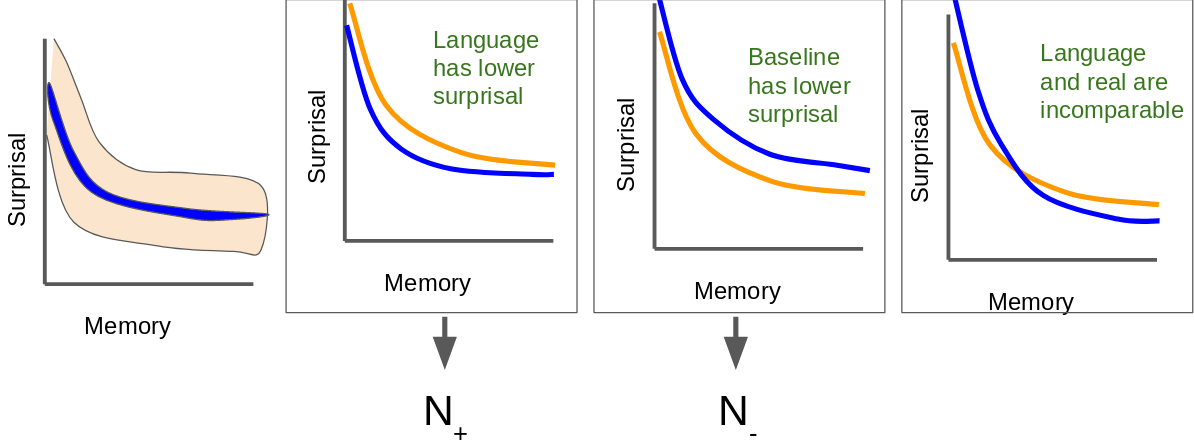
\includegraphics[width=0.8\textwidth]{figures/quantile-global.png}
\end{center}
	\caption{Illustration for the global quantile estimate serving as the stopping criterion. For each sample for the real language, we compare the memory-surprisal curve to all baselines.}\label{fig:quantile-global}
\end{figure}


For each language, we first collected 10 data points for real orderings and 10 data points for baseline orderings.
We continued obtaining new data points until the CI for $G$ had width $\leq 0.15$, or there were 100 samples from $P_1$ and 300 samples from $P_2$.
Up to the end, we chose the next sample to be from $P_0$ with probability 2/3, and $P_1$ otherwise.\footnote{Due to a scripting error, a much higher number of samples was generated for Erzya.}

This procedure was parallelized on several machines.
In the case where the stopping criterion was reached for a language while several machines were still computing samples for this language, we did not discard those samples.
Consequently, more samples were collected than necessary to reach the stopping criterion; however, in a way that does not bias our results towards or against our hypothesis.

%Due to parallelization of this procedure, it often produced more samples than required, when the stopping criterion .
%We chose these thresholds based on preliminary simulations which had suggested that these widths were achievable at acceptable computational cost.
%For each language, we collected at least 5 data points for real orderings and at least 10 data points for baseline orderings.
%We continued obtaining new data points until the CI for $G$ had width $\leq 0.15$, or there were 100 samples from $P_1$ and 300 samples from $P_2$.
%Up to the end, we chose the next sample to be from $P_0$ with probability 2/3, and $P_1$ otherwise.




\subsection{Results}



\begin{figure}
	\begin{center}
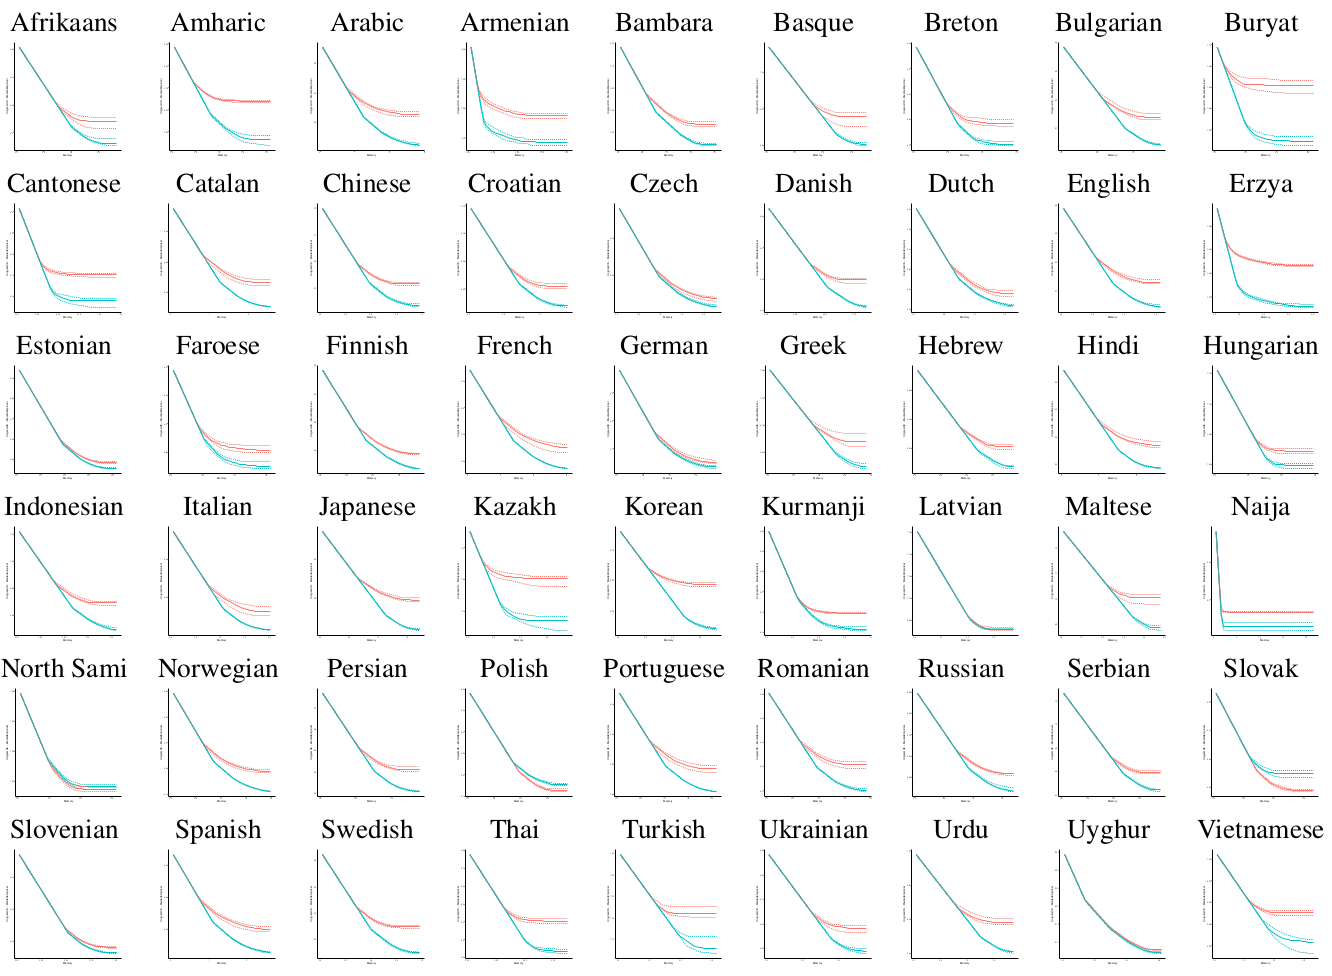
\includegraphics[width=\textwidth]{figures/full-results.png}
\end{center}
	\caption{Median surprisal (y-axis) at given memory level (x-axis), for real orders (blue) and random baseline grammars (red). We provide 95\% confidence bands. These are computed over different runs of the estimation algorithm for the real orders, and over different runs \emph{and} different grammars for the baseline grammars.}\label{fig:median-table}
\end{figure}



%The numbers of samples taken per language are provided in SI Table~\ref{tab:samples}.

%In Figure~\ref{tab:plain-results} (TODO), we show the estimated memory-surprisal tradeoff curves for all samples.


% yStudyTradeoff_Bootstrap_Parallel_OnlyWordForms_BoundedVocab_BinomialTest_Single_MedianCI.py
In Figure~\ref{tab:medians}, we show the median surprisal at given levels of memory, for real and baseline languages.
We compute surprisal at 40 evenly spaced points of memory (selected individually for each language), over all runs for the real language, and over all baselines grammars.
We then compute the median surprisal over all runs for the real language, and over all baselines grammars.
For each point, we compute a confidence interval for the median surprisal, using the binomial PDF. \mhahn{some standard stats reference}
This is an \emph{exact} confidence interval, without parametric assumptions or asymptotic approximations.

Numerically, the real language provides better tradeoffs than the median of the baselines across languages, with four exceptions (Latvian, North Sami, Polish, Slovak).

Bootstrapped confidence intervals for $G$ confirmed that $G>0.5$ in all but these four exceptional languages.

As bootstrapped confidence intervals are valid only asymptotically, we also conducted two \emph{exact} nonparametric tests to further ascertain the statistical robustness of this pattern.


At five evenly spaced memory values $\mu$ (chosen per language), we conducted a nonparametric and nonasymptotic significance hypothesis test against the null hypothesis that half of the baseline grammars have lower surprisal than the actual language. %(Figure~\ref{fig:nhst-pointwise}).
Formally, let $W_-(\mu)$ be the proportion of baseline languages that have strictly lower surprisal than the real language at memory level $\mu$.
For each level $\mu$ of memory, we consider the null hypothesis that
\begin{equation}
	W_-(\mu) = 0.5
\end{equation}
In this test, we approximate the surprisal value of the real language by the \emph{sample median}.
We use the Binomial Test.
We conduct a two-sided test.

In all but the four exceptional languages, the real language had significantly lower surprisal than at least $50\%$ of the baseline languages for at least some values of $\mu$ at $p < 0.01$.
Also, for those languages, there was no $\mu$ where this pattern was reversed.


%\subsection{Statistical Analysis}

%We now describe how we compared memory-surprisal tradeoffs between real and baseline languages.
%We want to test whether languages' surprisal-memory tradeoffs better than those of most baseline languages.
%We compare real and baseline languages by evaluating which languages result in lower surprisal at the same level of memory.
%We now describe the statistics we use to quantifying the difference between real and baseline languages.
%We do everything in a frequentist framework (null hypothesis testing \& confidence intervals), as we can do exact tests and confidence intervals without parametric assumptions.
%\mhahn{Maybe we can explain how the tests \& CIs also have reasonable Bayesian interpretations (for the specific methods used here, rejection of the null should guarantee that the posterior of the null hypothesis is small under a wide range of priors.).}

%\paragraph{Median Surprisal and Confidence Interval for Medians}



%\paragraph{CI for Median Difference}
%We create (nonparametric and nonasymptotic) confidence interval for the difference between real and baseline median surprisals at each memory value.
%\mhahn{the resulting plots are not very intuitive, might scrap this}
%
%% yStudyTradeoff_Bootstrap_Parallel_OnlyWordForms_BoundedVocab_BinomialTest_Single_MedianDiffCI.py



%This statistic also should have a reasonable Bayesian interpretation:
% E.g., if the random samples are unimodal, and we do inference over only the median (location family), 



%\begin{figure}
%	\begin{center}
%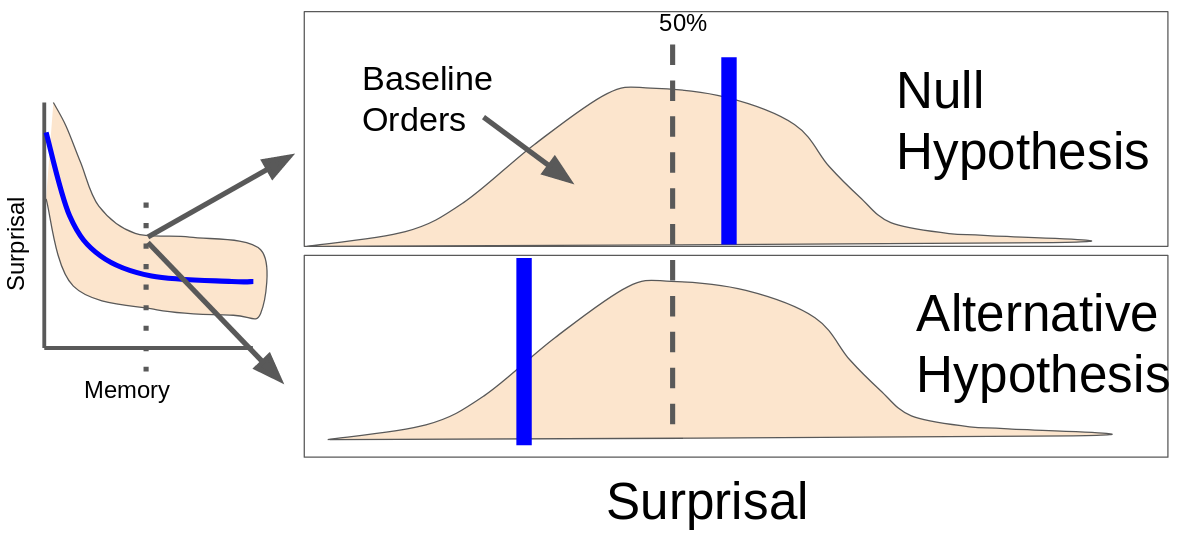
\includegraphics[width=0.45\textwidth]{figures/nhst.png}
%\end{center}
%	\caption{Illustration for the pointwise null-hypothesis significance test. At a given level of memory, we test against the null hypothesis that at least half of the baseline orders provide lower surprisal than the real language.}\label{fig:nhst-pointwise}
%\end{figure}






%For each memory value $\mu$, we do a significance test (nonparametric and nonasymptotic).
%\begin{equation}
%	W_+(\mu) \geq W_-(\mu)
%\end{equation}
%We use the empirical median for the real language.

% yStudyTradeoff_Bootstrap_Parallel_OnlyWordForms_BoundedVocab_BinomialTest_Single.py

%We take the REAL values to be estimated exactly by their medians.

In order to quantify the \emph{degree} of optimality, we compute what \emph{fraction} of baseline languages provides better tradeoffs than the real language.
%\paragraph{Pointwise Quantile Estimate}
%CI for quantile: % yStudyTradeoff_Bootstrap_Parallel_OnlyWordForms_BoundedVocab_BinomialTest_Single_UnimodalBoundOnQuantile_BothDirections.py
%\mhahn{might scrap the CI}
For each level of memory $\mu$, we estimate what percentage of baseline languages have lower (or equal) surprisal than the real language.
%This is described in Figure~\ref{fig:quantile-pointwise}.
We use the Binomial Test to derive a confidence lower bound for this quantile (CITE).
Again, we take the real values to be estimated exactly by their medians.

TODO some aggregate visualization of the quantiles

\paragraph{AUC}

TODO some aggregate visualization

%\begin{figure}
%	\begin{center}
%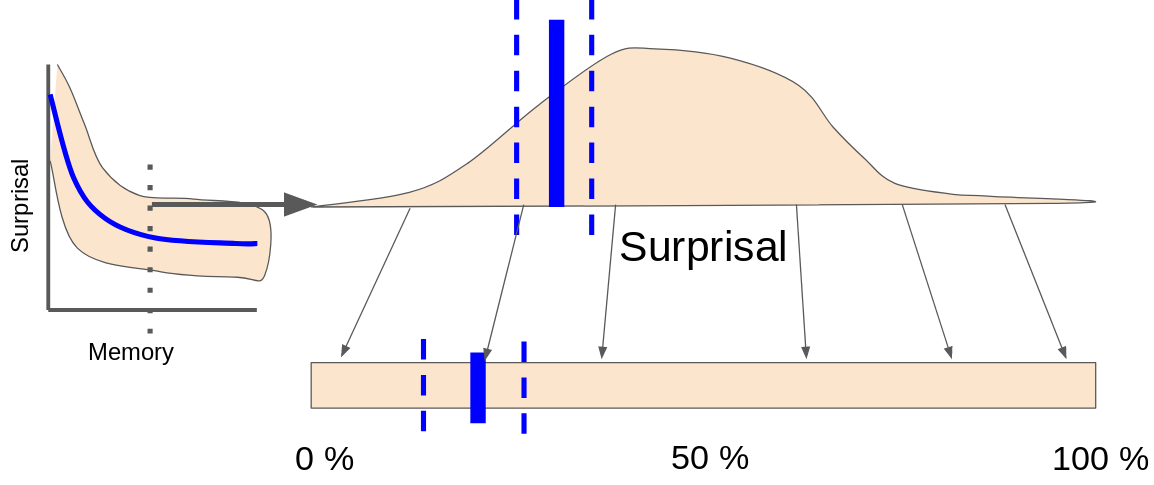
\includegraphics[width=0.45\textwidth]{figures/quantile.png}
%\end{center}
%	\caption{Illustration for the quantile estimate. At each level of memory, we provide an estimate of the percentage of baseline languages that have lower surprisal than the real language.}\label{fig:quantile-pointwise}
%\end{figure}



%Also the following does not assume unimodality, and ends up getting about the same intervals
%% yStudyTradeoff_Bootstrap_Parallel_OnlyWordForms_BoundedVocab_BinomialTest_Single_UnimodalBoundOnQuantile_BothDirections_NoAssumption.py






%In Figure~\ref{tab:slice-hists-real}, we show the distribution of surprisals achieved at the maximal memory value for real and random languages.

%In Figure~\ref{fig:hist-real}, we show surprisals at maximum memory, after z-transforming for each individual language and then aggregating.

%In Table \ref{tab:median_diffs}, we show the differences in median surprisal, as a function of memory.


%In Table~\ref{tab:boot-g}, we report the bootstrap estimates and confidence intervals for G~(\ref{eq:g}).
%$\E[G]$ was not estimated to be significantly above $>5$ for four languages: Latvian, North Sami, Polish, and Slovak.


%In Table~\ref{tab:quantiles}, we show the quantiles.





\subsection{Discussion}

We have found that 50 out of 54 languages provide better memory-surprisal tradeoffs than random baselines with consistent but counterfactual word order rules.

Four languages provide exceptions; these are Latvian (Baltic), North Sami (Uralic), Polish and Slovak (both Slavic).
All four languages have strong word order freedom (CITE).
Freedom of word order plausibly makes sentences less predictable, as the same syntactic structure can receive different surface realizations.
We thus hypothesized that freedom of word order impacts the memory-surprisal tradeoff, and that languages with more strongly fixed word order should display more optimal memory-surprisal tradeoffs.

To test this hypothesis, we examined the correlation between word order freedom and the surprisal difference between real and baseline orderings.
To quantify word order freedom, we used a corpus-based estimate, the \emph{branching direction entropy}~\citep{futrell-quantifying-2015}.
This is the entropy of the ordering (head-first or dependent-first) of dependencies conditioned on the dependency label and the part-of-speech label of head and dependent.
%\cite{futrell-quantifying-2015} showed that this me
These two quantities are plotted in Figure~\ref{fig:hist-real}.
We found that branching direction entropy was strongly correlated with the surprisal difference between real and baseline orderings (Spearman correlations -0.58, $p = 7.414e-6$).

We will address this in Experiment 3.


\begin{figure}
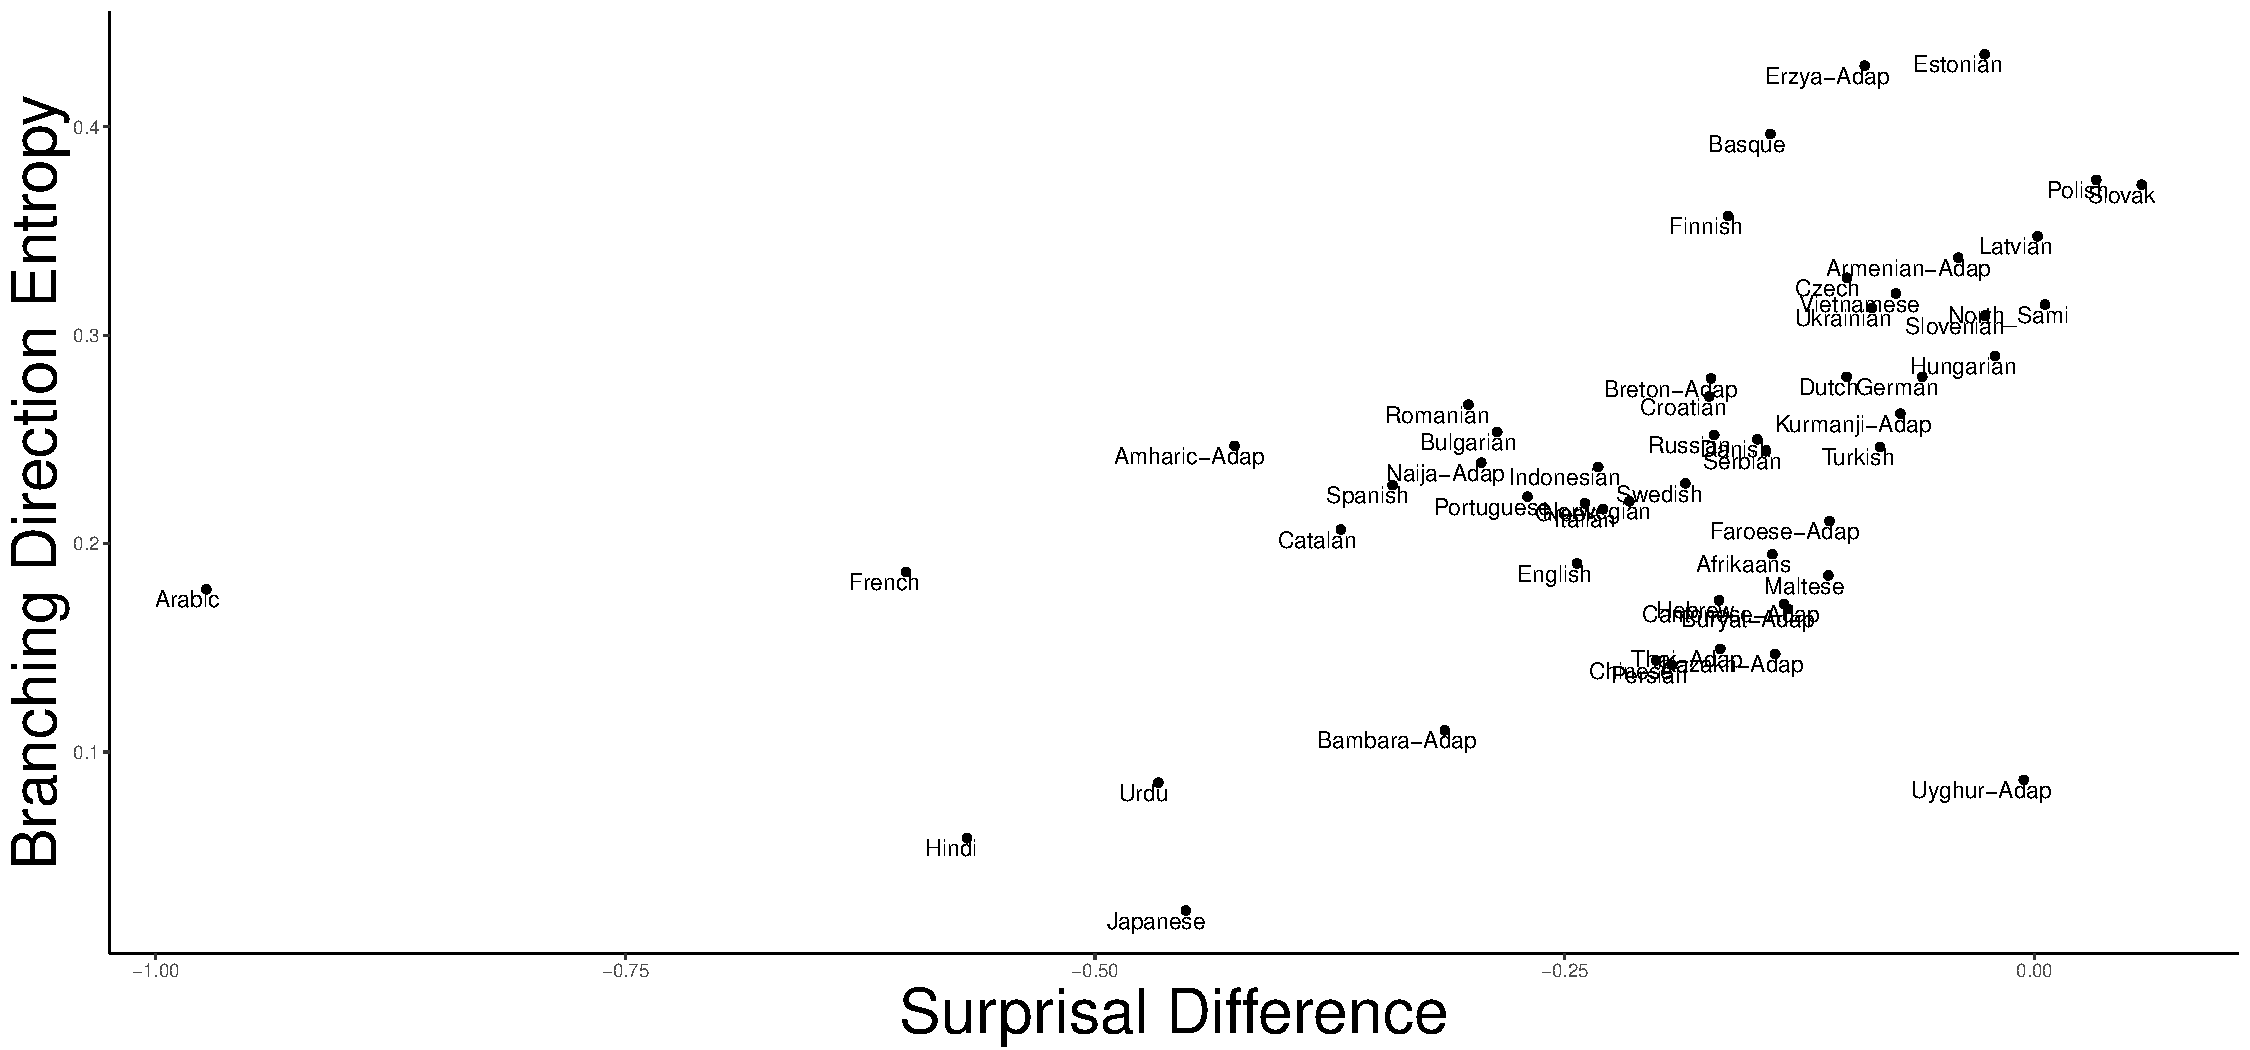
\includegraphics[width=0.95\textwidth]{figures/surprisal-branching-entropy-REAL.pdf}
	\caption{Surprisal Difference vs Branching Direction Entropy.}\label{fig:hist-real}
\end{figure}


\mhahn{One thing that has to be discussed: the absolute values differ between languages}



A possible concern is that the optimization observed in Experiment 1 might be an artifact of the grammar formalism.
We will address this in Experiment 3.
%To address this possibility, we repeated the experiment comparing baseline grammars to grammars that represent the word order of the real languages as faithfully as is possible with the grammar formalism.


